\chapter{Vers une théorie métabolique de la biogéographie des îles}
\label{chap4}



\section{Résumé en français du troisième article}

\subsection{Contexte scientifique}

Dans ce chapitre, je présente une formulation énergétique du modèle
de la TTIB \citep{Gravel2011}. Pour cela, je transforme l'île de la TIB en une
quantité de producteurs primaires. À partir de l'énergie générée par ces
derniers, je m'intéresse à la dynamique de colonisation de l'ensemble des
niveaux trophiques supérieurs du réseau écologique décrit à l'échelle régionale
(le metaweb tel que décrit aux chapitres précédents). Dans ce modèle, une espèce
du metaweb colonise une île sans difficulté si 1- elle y trouve une ressource
qu'elle est en mesure d'exploiter et si 2- il y a assez d'énergie disponible
pour que les espèces présentes puissent toutes maintenir une population locale
d'une taille minimale, si ces conditions ne sont pas remplies alors la colonisation
est impossible ou un processus d'extinction est enclenché. Je propose dans ce
chapitre un calcul simple mais astucieux pour intégrer les différences de
consommations entre les différents niveaux trophiques. Le calcul est
basé sur la biomasse des espèces mais aussi sur le transfert énergétique,
qui représente la quantité d'énergie qui passe d'un réseau à l'autre. À partir
de cette nouvelle formulation de la TTIB, j'obtiens une relation espèce-énergie
(SER) informative sur la structure du réseau.

L'approche que je propose est, à mon avis, un pas significatif vers une
intégration plus aboutie des mécanismes écologiques dans la TIB, notamment pour
les interactions biotiques. Je prolonge le travail de la TTIB et
je fais un premier rapprochement avec la théorie métabolique de l'écologie.
Bien que le modèle proposé soit relativement simple, il est une pierre solide
pour aller plus loin dans l'exploration d'une théorie métabolique de la
biogéographie. De plus, au regard de l'abondante littérature relative aux
relations allométriques, il me semble essentiel de comprendre comment les
contraintes énergétiques, exercées à l'échelle de l'individu,
se propagent à l’échelle des populations puis aux échelles biogéographiques.



\subsection{Publication envisagée}

Présentement, l'article offre des perspectives intéressantes sur une
théorie métabolique en biogéographie mais aussi des pistes de réflexion
pour s'affranchir simplement de certaines contraintes de modélisation
qui pourraient hautement complexifier le modèle (par exemple, je ne considère
pas explicitement la dynamique des populations sur l'île). Je vois deux opportunités
associées au travail ici présenté. Premièrement, orienter davantage mon travail
sur les aspects techniques et mathématiques du modèle et essayer,
par exemple, de dériver une solution approchée du modèle.
Cela m'orienterait vers une publication plus technique
pour un journal spécialisé sur les aspects théoriques en écologie. Deuxièmement,
aller plus loin dans l'exploration des possibilités offertes par le modèle,
insister sur les perspectives, notamment sur l'impact de la structure des
réseaux sur la relation énergie-espèces. Cela m'orienterait plutôt vers
un article de perspectives, pour un journal d’écologie généraliste.

Pour cet article ma réflexion a été alimentée par discussion avec Dominique
Gravel, Miguel Araújo et Loïc Pelissier que je remercie. Je me suis occupé de
concevoir le modèle, d'implémenter le modèle et de sortir les résultats et de
l'analyser. J'ai écrit la première version du modèle et j'ai bénéficié d'apports
significatifs de Dominique Gravel qui a fait une relecture complète du
manuscrit. Je remercie également chaleureusement Kevin Solarik qui m'a apporté
de nombreuses relectures mais aussi des suggestions pertinentes. Cet article est
également la base de réflexion du travail que j’aimerais mener dans un projet
de recherche post-doctoral.



\subsection{Traduction du résumé en anglais}

L’énergie façonne la biodiversité; l’abondance de l’énergie solaire et la
disponibilité en eau décrivent bien les écosystèmes terrestres de même que la
température de surface de la mer et la disponibilité en nutriments écrivent les
écosystèmes marins. À l'échelle de la communauté, les réseaux trophiques et
leurs structures déterminent les échanges d'énergie des producteurs primaires
jusqu'aux prédateurs du haut de la chaîne alimentaire. En dépit de sa grande
importance, l'introduction de l'énergie dans les théories classiques en
biogéographie a été négligée, ces théories considèrent les espèces équivalentes
(c'est le cas de la Théorie de la Biogéographie des Îles) ou se concentrent sur
le concept de niche écologique. Pour rectifier cela, nous développons une théorie
pour inclure les contraintes énergétiques pour décrire la répartition de la biodiversité.
Comme illustration des perspectives offertes par cette approche, nous étudions
la richesse spécifique et la structure des réseaux le long d'un gradient
d'énergie. Avec l'augmentation de l'énergie disponible, nous obtenons une succession claire
des espèces selon leur statut trophique~: des plus bas niveaux trophiques sur
les îles pauvres en énergie jusqu'aux plus hauts niveaux sur les îles où l'énergie
est abondante. C'est une piste prometteuse pour aller au-delà de la prédiction quantitative
des pertes d’espèces lorsque les habitats sont fragmentés et prédire le rôle qu'elles
ont au sein du réseau écologique. Nous pensons que l'utilisation de ce modèle
sera très utile pour une intégration de l'écologie des communautés en biogéographie,
tout en permettant aussi une meilleure paramétrisation des modèles de distribution
d'espèces.




\emph{Les sections qui suivent sont celles de l'article publié.}
\section{Title}\label{title}

Towards a metabolic theory of island biogeography.


\section{Abstract}\label{abstract}

Energy availability shapes biodiversity; solar radiation and water
availability describes the terrestrial ecosystems well, just as sea
surface temperature and nutrients availability describe marine
ecosystems. At the community scale, food webs and their structures
control energy exchanges from primary producers to top predators.
Despite its crucial importance, the implementation of energy has been
overlooked in classical theories in biogeography, which often assume
species are equivalent (\emph{e.g.} the Theory of Island Biogeography) or
either remain too focused on the concept of the ecological niche. In
order to rectify this, we develop a theory to include energy constraints
to describe the distribution of biodiversity. As an illustration of the
perspectives offered by this framework, we derive expected species
richness and network structure along an energy gradient. When increasing
the energy availability, we obtain a clear succession of species
according to their trophic status, from the lowest trophic level on poor
energy islands to the highest species when energy is abundant. This a
promising avenue to predict more than a expected number of species we
loss when habitat is fragmented but also their role in the ecological
network. We are confident the use of this model will be proven
beneficial for the integration of community ecology with biogeography,
while also better parameterize species distribution models.

\section{Introduction}\label{introduction}

Disentangling the relative contribution of the different processes
shaping biodiversity distribution is the central objective of
biogeography. While biogeographers clearly envision the list of
ingredients needed to understand species distribution
\citep{Thuiller2013}, they miss the framework to mix them in the right
amount and to investigate the biogeography of ecological communities. We
will likely fail to predict accurately biodiversity responses to global
changes as we keep our focus strictly on abiotic factors \emph{i.e}
temperature and precipitation, while continuing to overlook biotic
interactions \citep{Wiens2011} and short-term evolutionary responses
\citep{Lavergne2010}. At the core of this issue is the need for an
integrated approach at the crossroad between species distribution
modelling and community ecology.

Biotic interactions should be integrated as a constraint for species
co-distribution in meta-communities \citep{Jabot2012, Cazelles2016a}.
Ecological interactions may explain, at least partially, the dynamics of
local extinctions, which in turn would further explain some properties
of the geometrical shape of species ranges \citep[\emph{e.g.} nested
distributions of parasitoid and its host,][]{Shenbrot2007}. We have
however limited evidence of the effect of biotic interactions on large
scale species distribution \citep[see Chapter \ref{chap3} - but
see][]{Gotelli2010}. Incidentally, two of the most influential models in
biogeography assume ecological equivalence of species; the Theory of
Island Biogeography of MacArthur and Wilson \citep[hereafter
TIB,][]{MacArthur1967} overlook the variation among species
characteristics and ignore their arrangement in organized ecological
networks. In his neutral theory, Hubbell assumes that individuals of
different species are ecologically equivalent and predicts the
distribution of abundance without considering interactions
\citep{Hubbell1997, Hubbell2001}. These two theoretical models have been
proven relevant for certain groups of species and inadequate for others,
and none of them were initially intended to describe exhaustively the
structure of ecological communities. The integration of ecological
interactions into biogeography however offers promising perspectives and
a much extended range of predictions \citep{Holt2010, Gravel2011}.

The TIB is well-suited to explore the consequences of ecological
interactions on community structure at broad spatial scales, as it
includes two fundamental processes of biogeography, immigration and
extinction, in an elegant fashion that eases its extension
\citep{Losos2010, Warren2015}. Building upon the classical model of
MacArthur and Wilson, recent studies have included various forms of
interactions in the TIB \citep{Gravel2011, Cazelles2016a}. The regional
species pool becomes a \emph{metaweb}, not only listing potential
colonists but also their interactions. With this approach, species are
inter-dependent entities with specificities (\emph{e.g.} a given trophic
level) rather than indistinguishable units. As a consequence,
colonization and extinction rates vary with respect to species identity
\emph{and} the composition of the local community. \citet{Gravel2011}
proposed the Trophic TIB (hereinafter TTIB) to represent food web
assembly on isolated communities, where predators can persist locally as
long as they find at least one preys. More generally,
\citet{Cazelles2016a} presented a Lotka-Volterra like model in which the
composition of the local community determines both colonization and
extinction rates. Adding new ecological processes in the TIB increases
realism, at the cost however of reducing its simplicity. It provides an
extended list of predictions, which have yet to be proven significantly
better than the original theory \citep[see][]{Cirtwill2015}. Extending
the TIB while preserving its elegance is a challenging and technical
issue. Here we propose to reformulate the TTIB in terms of energetic
constraints in attempt to solve this challenge.

The TIB was originally meant to predict and explain the common
observation of increasing species richness with island area. Another
ubiquitous and fundamental observation in biogeography is the
latitudinal diversity gradient
\citep[LDG,][]{Rhode1992, Stevens1989, Evans2005}. The productivity of
primary producers is generally found the best predictor of species
richness at large spatial scales \citep{Evans2005, Storch2005}. Others
found a strong correlation between richness, water availability and
temperature \citep{Currie1993, Hawkins2003}. Several mechanisms have
been proposed to explain this relationship \citep[see][ for a
review]{Currie2004, Evans2005}, including higher speciation rates in
tropical areas, greater biomass and finer niche partitioning. Recently,
some authors investigated how networks could change with latitude. Based
on the meta-analysis of 196 empirical food webs, \citet{Cirtwill2015a}
shown that ecological networks of interactions also vary along this
gradient but that the density of links remains constant throughout. In
the majority of ecosystems theses authors studied, an increased energy
results in a wider niche space, rather than an increase of niche breadth
poleward. Similarly, \citet{Albouy2016} reconstructed marine networks
across the globe and found significant latitudinal-network gradients
(LNG). These studies are however descriptive only, as there is currently
no theory to explain how and why energy constraints should impact food
web structure. In 1983, \citet{Wright1983} developed the species-energy
theory and replaced the ``area'' with ``available energy'' to derive a
meaningful Species Energy Relationship (SER). Although area and energy
may bring more information taken together \citep{Storch2005}, the
rationale behind it allows the derivation of species abundance and
occurrence probability based on energetic constraint \citep{Wright1983}.
Wright's approach however do not specifically account for network
structure and thereby remains limited to species richness.

Species do not escape from the laws of thermodynamics and as a
consequence, despite the complexity of evolutionary trajectories, many
key ecological properties and processes scale with body mass
\citep[\emph{i.e.} metabolic theory of
ecology][]{Brown2004, Woodward2005a}. The scaling of the metabolic rates
with body mass is the fundamental observation underlying this theory
\citep{Gillooly2001}, which typically follows a power function with
coefficients often between 2/3 and 3/4 \citep{White2013}. Even if all
the relationships are not well-understood \citetext{\citealp[see the
case of abundances reviewed in][]{White2007}; \citealp[and the recent
relationship between prey and predator biomasses][]{Hatton2015}}, the
ubiquity of allometric relationships makes body mass distribution a key
variable to reduce the complexity of ecosystems. Allometric
relationships and energy flows also provide the mean to parameterize
models of population dynamics \citep{Yodzis1992}. Recent developments of
food web theory have convincingly shown that allometric relationships
are the cog to analyze the properties of ecological networks
\citep{Gravel2013, Petchey2008}, their dynamics \citep{Brose2006} and to
characterize the role of species within them \citep{Schneider2012}.

Our objective in this study is to develop a theory of biodiversity
distribution based on first principles of energetic constraints in order
to investigate the impact of trophic interactions on the
latitudinal-diversity gradient. We propose to extend the model of the
TTIB following the vision of \citet{Wright1983}. As a consequence, our
theory encompasses both the species-area and the species-energy
relationships, making it a very general framework to understand and
predict biodiversity distribution. In addition, the explicit integration
of trophic interactions allows the development of a vast array of
testable and insightful predictions, including the expected
latitudinal-network gradient. To do so, we propose a theoretical model
of food web assembly driven by colonization from the regional metaweb
and energetic constraints. We derive expected species richness and
network structure along gradients of primary productivity. We use
``Lindeman'' \citep{Lindeman1942} transfer efficiency (\emph{i.e.}
energy transferred to another trophic level) to integrate
species-specific differences in their source of energy. We derive a SER
and the relationship between body-mass distribution and available
energy. Our model formalizes the initial hypothesis of Lindeman and
offers immense possibilities for the integration of community ecology
with biogeography.

\section{Model description}\label{model-description}

The model developed by MacArthur and Wilson predicts species richness on
an island according to the size of the island and its distance from the
mainland \citep{MacArthur1967}. One promising direction to extend this
theory is to include biotic interactions into the classical model
\citep{Holt2010, Gravel2011, Cazelles2016a}. Following this avenue, we
consider explicit interactions among the regional pool of species based
on allometric relationships. Body mass is used to determine the quantity
of energy a given species requires to maintain its local population on
an island. Extinction follows if the island cannot sustain a minimal
population of any given species. Therefore, in the model described
below, we simulate the TIB with purely stochastic colonization events
together with deterministic extinction based on an energy rational.

We consider an island as an isolated piece of land covered by a maximal
quantity of primary producers, which determine the amount of available
energy upon which a food web can develop. We denote \(E_0\) the maximal
amount of energy available for herbivores and consider it to vary
proportionally to island area. Here we do not enter the specificities of
how productivity scales with area, as in some situation it could scale
linearly or not \emph{e.g.} for lakes when the volume determines
productivity \citep{Post2000}. As a consequence, the model explains both
the scaling of richness with island area and productivity, with the same
underlying principle that a minimal population size is required for
persistence. We make two additional simplifications: the diversity of
primary producers is not taken into account, and the production is
constant over the time.

The regional pool of species in the TIB is the number of species \(P\)
and the tropic interactions among them. Following \citet{Cazelles2016a},
potential interactions among them are determined using the niche model
\citep{Williams2000}. We furthermore assume the niche axis to be the
body size of the species \citep{Gravel2013} and that species which are
without any links in the metaweb are determined to be herbivores. Note
that primary producers are not included in the niche model but the
source of energy of herbivores. They are rather included in the total
energy \(E_0\) (see below) consumed by herbivores. As a consequence,
trophic level is strongly correlated to body mass, with herbivores often
the smallest and top predators the largest. Although this assumption is
an oversimplification of the determinants of ecological interactions, it
remains reasonable for marine ecosystems \citep{Trebilco2013}, where
allometric relationships have been used to infer food web structure
\citep{Gravel2013}.

Following \citet{Gravel2011}, we assume that the colonization of
herbivores/predators is successful only if they find at least one of
their habitat/prey on the given island. Additionally, we propose that
colonization events are possible only if the energetic requirements to
maintain local populations exceeds the primary production. In this case,
energetic constraints and network topology determine the identity of
species to go extinct. Colonization events are assumed to be purely
stochastic, while extinctions are deterministic, control by the
energetic constraints \citep[this difference in stochastic nature
between these fundamental processes of biogeography has been recently
supported in][ where the authors show that extinction probability
decreases with the presence of resource/prey on the
island]{Cirtwill2015}.

\subsection{Energetic constraints on local food
webs}\label{energetic-constraints-on-local-food-webs}

The rational for energetic constraints is simple: local populations need
a certain amount of energy to maintain a minimum level of activity
otherwise they die from starvation. Under this constraint, species
richness locally increases until the energy available on the island
(\(E_0\)) is no longer sufficient for all populations because of
inefficient energy transfer at each trophic interactions. Therefore all
population on the island are maintained as long as the inequality below
holds true:

\begin{equation} \sum_i e_i \leq E_0\label{eq:chp4id0}\end{equation}

where \(e_i\) is the energy uptake of the insular population of species
\(i\). We now need to define a rule to set the the minimal energy a
population needs to survive on the island. For a given species \(i\),
energy requirements of any individual is derived from allometric
relationships proposed by the metabolic theory of ecology
\citep{Brown2004}, of the form \(c_im_i^b\) where \(c_i\) is a constant,
specific constant, \(m_i\) the body mass of species \(i\) and \(b\) the
coefficient of power \citep[between 2/3 and 3/4][]{White2013}. We do not
integrate intraspecific variability in body mass and thus \(m_i\) is a
constant for a species. The energy uptake associated to a minimal viable
population (hereafter MVP) of \(n_i\) individuals becomes \(n_im_i^b\).
\citet{Shaffer1981} defined the MVP as ``\emph{{[}\ldots{}{]} the
smallest isolated population having a 99\% chance of remaining extant
for 1000 years despite the foreseeable effects of demographic,
environmental and genetic stochasticity, and natural catastrophe}'',
highlighting that the smallest portion of a population has the highest
possible extinction risk (extrapolated as time to extinction). The key
problem is wether or not the MVP is size dependent. The most
conservative assumption is to consider it to be a constant.
\citet{Lande1993} however shown that the time to extinction is affected
by the mean population growth rate, which underlies that species
characteristics may lead to a heterogeneity in MVP. Moreover,
\citet{Savage2004} had developed a framework within which they proved
the growth rate to be proportional to \(m_i^{-b}\). Based on these
results, we explore two different rules for extinctions: (1) MVP is
equal for all species: \(n_i=n_0\), and (2) MVP scales with the growth
rate \(n_i=n_0m_i^{-b}\). For both scenarios, species \(i\) can survive
only if the energy expenditures can be covered, \emph{i.e} if the energy
available is greater than: \(n_ic_im_i^b\).

\subsection{Energy fluxes and transfer
efficiency}\label{energy-fluxes-and-transfer-efficiency}

Although the expression of energy consumption is similar among species,
they obtain it from different sources: herbivores feed on primary
producers, whereas predators feed on a set number of secondary
consumers. The primary production must therefore be tracked as it moves
up through the food chain. To deal with this, we propose to convert the
energy costs for maintaining predator populations into additional
populations of herbivores to be maintained. To exemplify this idea, we
start with the simplest trophic network where a predator \(j\) feeds
upon a herbivore \(i\). The cost to maintain the MVP of \(i\) is
\(n_ic_im_i^b\) and \(n_jc_jm_j^b\) for \(j\). For the latter, we
convert \(n_j\) into an extra population of \(i\), \(n_{i,j}\) herbivore
individuals dedicated to \(j\) consumption. Furthermore, we account for
the energy loss during consumption by including a transfer efficiency
\citep[sensu][]{Lindeman1942} \(\tau\). Hence, the conversion from
\(n_{j}\) to \(n_{i,j}\) is given by the following equation:

\begin{equation} \tau n_{i,j} c_im_i^b = n_jc_jm_j^b \label{eq:chp4id1}\end{equation}

the energy requirements of \(n_j\) are converted into a energy expressed
in term of a population of \(i\) based on which we obtain the population
size of \(i\) needed to maintain a MVP of \(j\):

\begin{equation} n_{i,j} = \frac{n_jc_j}{\tau c_i} \left( \frac{m_j}{m_i} \right)^b \label{eq:chp4id2}\end{equation}

We postulate that the transfer efficiency is constant across trophic
levels, which is likely an oversimplification of the reality as
suggested by the sparse empirical data available
\citep{Trebilco2013, Brown2003}. We now add a new predator \(k\) feeding
on \(j\) (the predator of \(i\)) to the insular food web. According to
our reasoning, we must covert \(n_k\) into \(n_{i,k}\). To do so, we
start by converting \(n_k\) into a population of \(j\):

\begin{equation} n_{j,k} = \frac{n_kc_k}{\tau c_j} \left( \frac{m_k}{m_j} \right)^b \label{eq:chp4id2}\end{equation}

We now turn \(n_{j,k}\) into a herbivore population:

\begin{equation} n_{i,k} = \frac{\frac{n_kc_k}{\tau c_j} \left( \frac{m_k}{m_j} \right)^bc_j}{\tau c_i} \left( \frac{m_j}{m_i} \right)^b \label{eq:chp4id3}\end{equation}

which gives:

\begin{equation} n_{i,k} = \frac{n_kc_k}{\tau^2 c_i} \left( \frac{m_k}{m_i} \right)^b \label{eq:chp4id3b}\end{equation}

In a similar fashion, for a linear trophic chain, we can demonstrate
that the additional population of herbivore \(i\) necessary to maintain
predator \(j\) of level \(l\) is:

\begin{equation} n_{i,k} = \frac{n_jc_j}{\tau^l c_i} \left( \frac{m_j}{m_i} \right)^b \label{eq:chp4id4}\end{equation}

In many cases, a predator feeds on an array of prey species rather than
a single one. As such, it uptakes its energy from the different sources
and we must account for all of them. We assume that energy costs
associated with maintaining the local predator are minimal. Therefore,
\(n_j\) is converted into \(i\), the herbivore linked to \(j\) for which
(\ref{eq:chp4id4}) is minimal. Basically, \(i\) should be a large and
separated from \(j\) by a low number of species. Hence, on the island,
the species richness increases as long as the inequality below holds
true:

\begin{equation} \sum_i c_in_im_i^b + \sum_j \frac{n_jc_j}{\tau^{l_j} c_i} \left( \frac{m_j}{m_{i_j}} \right)^b \leq E_0 \label{eq:chp4id5}\end{equation}

The first term is the energy cost for maintaining populations of
herbivores, the second term is associated to higher trophic levels:
predator \(j\) is converted into herbivore \(i_j\) from which it is
separated by \(l_j\) links. For the sake of simplicity, we make an extra
assumptions: \(c_i\) values are constant among species and set to 1.
Therefore, if we assume that MVP is constant (scenario 1), inequality
\ref{eq:chp4id5} becomes:

\begin{equation} \sum_i m_i^b + \sum_j \frac{1}{\tau^{l_j}} \left( \frac{m_j}{m_{i_j}} \right)^b \leq \frac{E_0}{n_0} \label{eq:chp4id5a}\end{equation}

Similarly, if we assume \(n_i=n_0m_i^{-b}\) and \(n_j=n_0m_j^{-b}\)
(scenario 2), then:

\begin{equation} \sum_i 1 + \sum_j \frac{1}{\tau^{l_j}} \left( \frac{1}{m_{i_j}} \right)^b \leq \frac{E_0}{n_0} \label{eq:chp4id5b}\end{equation}

The left side of this equation provides the minimal energy needed to
sustain all populations while the right side is the total amount of
energy available. Therefore, the maximal population of species \(i\)
without any extinction is given by converting the extra amount of energy
available into an additional population of species \(i\), the population
of \(i\) we get is denote \(n_{i,max}\). The range \([n_i, n_{i, max}]\)
is then the range of possible fluctuations of species \(i\) without any
new extinction event.

\subsection{Extinctions}\label{extinctions}

When the local primary production cannot sustain the establishment of a
new immigrant, \emph{i.e.} when inequality \ref{eq:chp4id5} is no longer
verified, its arrival is either impossible or lead to extinction of
other species. In the latter situation, we must determine the identity
of species that will go extinct, which remains a significant challenge
that will not be undertaken here given its complexity highlighted by
recent theoretical studies \citep{Saterberg2013, Zhao2016}. To overcome
this concern, we use two scenarios: (1) \emph{random extinction}: any
species can go extinct, and (2) \emph{costs-based extinctions}: the
probability of extinction is proportional to the energetic costs of the
species. Once an extinction occurs, we ensure that all species remain
linked to at least one herbivore, otherwise unlinked species will too go
extinct. Finally, extinctions are set to occur until \ref{eq:chp4id5} is
satisfied. Note that the deterministic nature of extinctions lays in in
the fact that they occur when energy is lacking, the identity of the
species that actually goes extinct remains stochastic.

% \begin{table}[]{@{}lll@{}}
% \caption{Hypotheses associated to the four scenarios.
% \label{tbl:scena}}\tabularnewline
% \toprule
% Scenario & MVP & extinction\tabularnewline
% \midrule
% \endfirsthead
% \toprule
% Scenario & MVP & extinction\tabularnewline
% \midrule
% \endhead
% A & \(n_0\) & random\tabularnewline
% B & \(n_0\) & costs-based\tabularnewline
% C & \(n_0m^{-.75}\) & random\tabularnewline
% D & \(n_0m^{-.75}\) & costs-based\tabularnewline
% \bottomrule
% \end{longtable}

\begin{table}
  \centering
  \caption{Hypotheses associated to the four scenarios.
  \label{tbl:scena}}
  \begin{tabular}{lll}
    Scenario & MVP & extinction \\ \hline
    A & \(n_0\) & random \\
    B & \(n_0\) & costs-based \\
    C & \(n_0m^{-.75}\) & random \\
    D & \(n_0m^{-.75}\) & costs-based
  \end{tabular}
\end{table}


Although the assumptions we have made here are likely unrealistic, our
intentions are merely to examine the model under the special case of an
optimal energy allocation on an island. These assumptions remain
acceptable as long as we focus on the qualitative consequences in term
of community dynamics. As an important remark, the energy cost
associated to one predator is not based on inherent properties only, as
it is determined also by the identity of its preys present on the island
(in other words, via apparent competition). Hypotheses made for the four
scenario are recapitulated in Table \ref{tbl:scena}.

\begin{figure}[htbp]
\centering
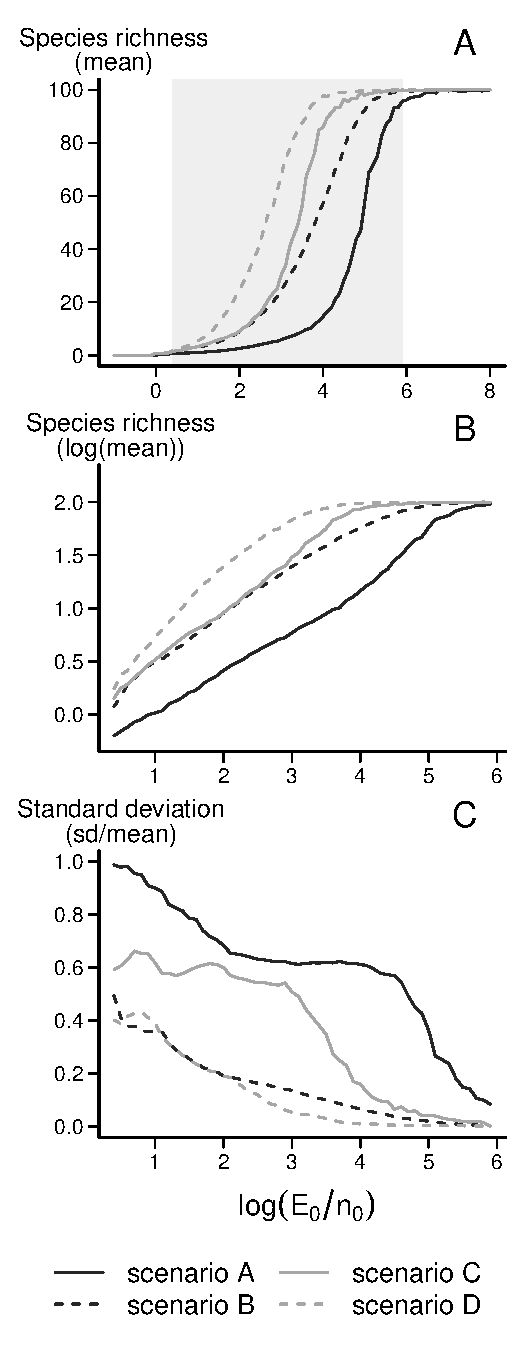
\includegraphics[width=0.5\textwidth]{chapitre4/fig/fig1.pdf}
\caption[Species-Energy Relationship]{\textbf{Species-Energy Relationship} using 100 replicates for
each of the four scenarios for (A) mean species richness, (B) logarithm
of the mean, and (C) coefficient of variation.\label{fig:etib1}}
\end{figure}

\subsection{Simulations}\label{simulations}

Every simulation starts with the generation of the regional metaweb of
100 species. To do so, we first draw a number \(p_i\) for all species
from a uniform distribution from the range {[}0,3{]}. Numbers \(p_i\)
are then sorted, the lowest values are assigned to the herbivores and we
use the vector obtained as the niche axis in the niche model, with
connectance set to \(0.05\) \citep{Williams2000}. Species that are not
connected are assumed to be herbivores and to allow comparisons among
simulation we standardize the number of herbivore to 10. To do so we
keep generating new metawebs until one we obtain one metweb with 10
species that were not connected. We also use the \(p_i\) number to
derive the biomass of all species, we do so by using \(10^{p_i}\). The
smallest species has the smallest niche axis.

We simulated the model along a gradient of energy ranging in
\(\frac{E_0}{n_0}\) from \(.1\) to \(10^8\). We start with an empty
island and at any time step, any species of the metaweb has a
probability \(c=0.001\) of colonizing the island. If a successful
colonization occurs if available energy on the island allow to sustaint
a MVP of the new species. For all time step we record the species on the
island. We perform 125,000 iterations and discard 25,000 burn-in
iterations and the 100,000 remaining to do our analyses. For all the 91
values of the energy gradient we used 100 replicates, meaning 100
different regional metawebs.



\section{Results}\label{results}

We found a sigmoidal SER for all scenarios (Fig. \ref{fig:etib1} A).
Under scenario A, for instance, species richness increased exponentially
with the increase in energy, where more species were allowed to colonize
the island (Fig. \ref{fig:etib1}). SER reached saturation much faster
under scenarios C and D than under the scenarios A and B, due to the
difference in energy uptake. Under scenarios C and D the MVP decreased
with body mass, which allows higher species richness or a comparable
amount of energy. Remarkably, species richness was smaller for scenarios
where the extinction rate was cost-based than randomly based (Fig.
\ref{fig:etib1} A-B), which also results in less variability (Fig.
\ref{fig:etib1} C).

\begin{figure}[htbp]
\centering
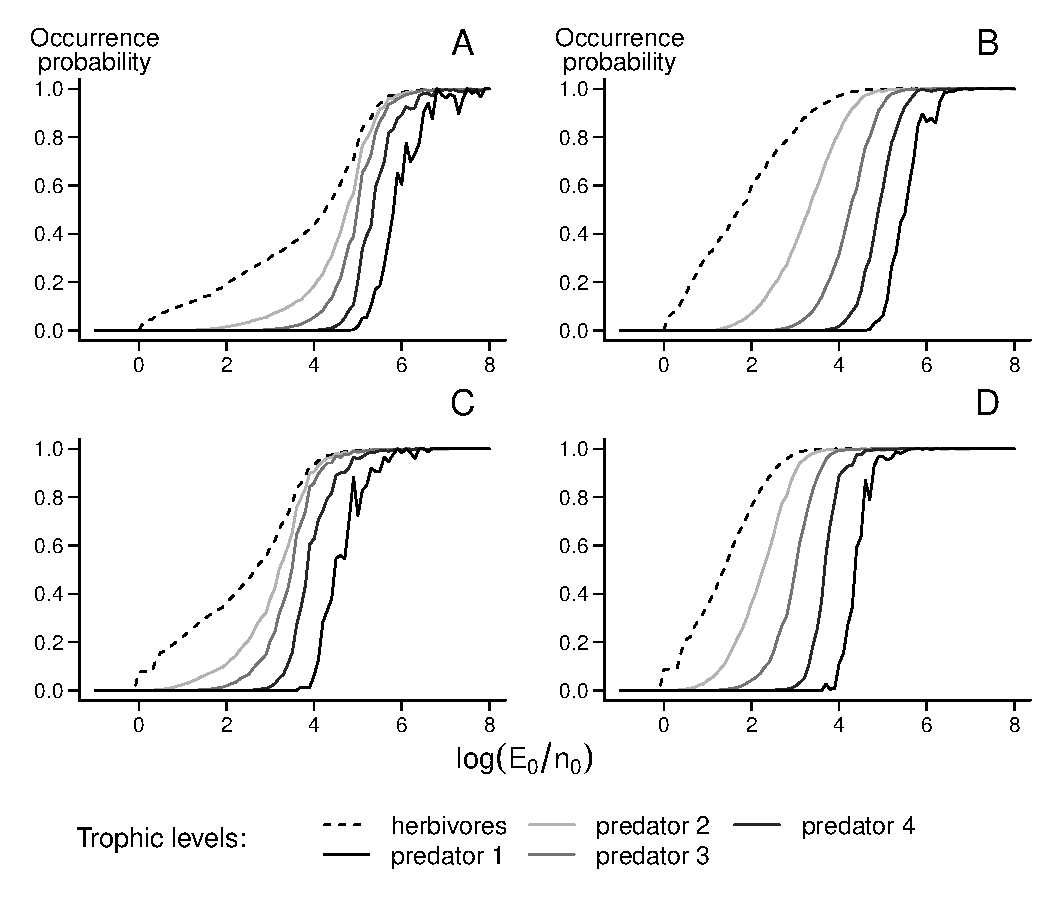
\includegraphics[width=\textwidth]{chapitre4/fig/fig2.pdf}
\caption[Species occurrence probability along an energy
gradient, grouped by trophic level]{\textbf{Species occurrence probability along an energy
gradient, grouped by trophic level}; herbivores, or by their shortest
path linking to a herbivore species. The top right letters indicates the
scenarios.\label{fig:etib2}}
\end{figure}


Occurrence probability increases with available energy and decreases
with trophic level for all scenarios (\ref{fig:etib2}). Herbivores were
found to colonize the island first, followed by predators of increasing
trophic level. The trend was similar for all scenarios, and more
pronounced for those where extinction is cost-based (scenarios B and D).
When species occurrence probabilities were grouped by body mass, only
significant differences were found within scenario B (\ref{fig:etib3}).
Taken together, these results highlight the importance of network
structure. Here, we outline the importance of colonization, where the
shortest path between herbivore and predator is extremely important
especially given it strongly impacts the cost of a species; suggesting
that this is the cause of the main differences among random and
cost-based extinction rates.


The average species body mass increased with energy under scenarios A
and B, but decreased under scenarios C and D. The reduction of MVP with
body mass would therefore allow for larger species to maintain on small
island (\ref{fig:etib4} A-D). We see a similar trend for the number of
prey species, which increases with energy in scenarios A and B, while it
decreases in scenarios C and D (\ref{fig:etib4} E-H). Ultimately,
generalist species have a much higher rate of successful colonization
under low energy in scenarios C and D. When the MVP is smaller, larger
species can colonize and their probability of success is higher as they
have more preys in average \citep[due to the use of the niche model and
body mass as the niche axis][]{Williams2000, Gravel2013}. Finally, under
scenarios A and B small species with several predators colonize low
energy islands while under scenarios C and D the same species colonize
the island with higher energy availability as they are preceded by
larger and more generalist species (\ref{fig:etib4} I-L). Consequently,
the number of interactions per species increases faster under scenarios
C and D than under scenarios A and B (\ref{fig:etib4} M-P).

\begin{figure}[htbp]
\centering
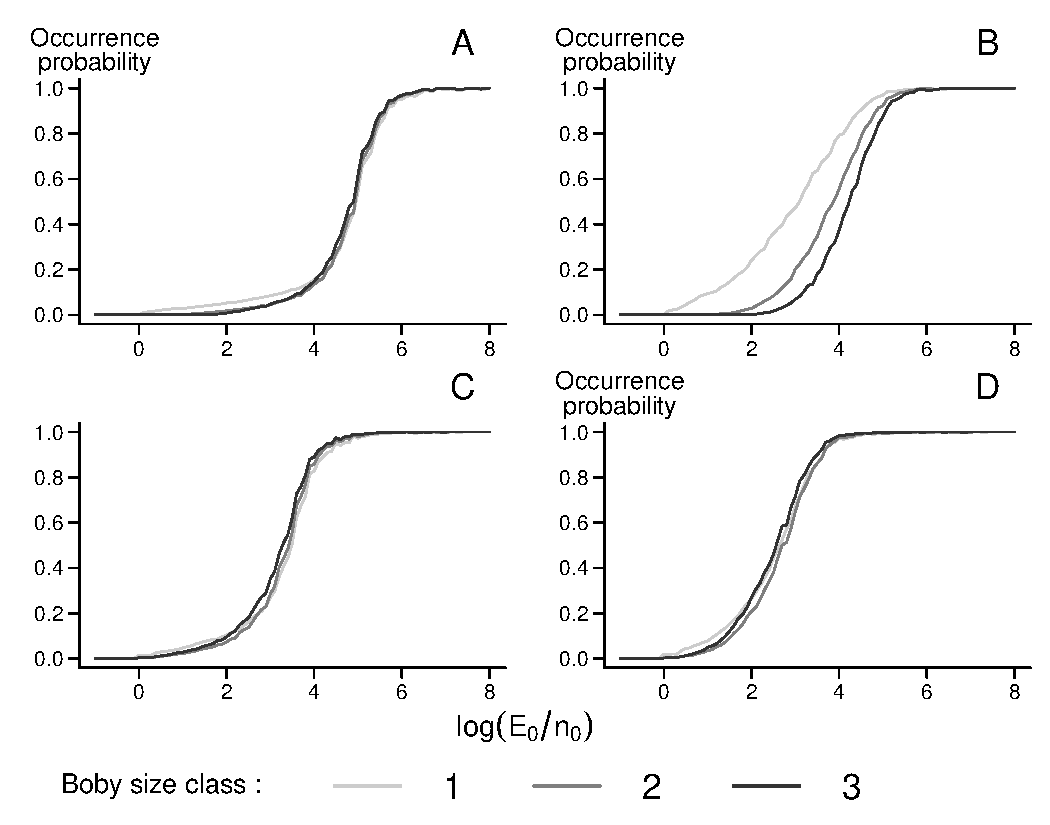
\includegraphics[width=\textwidth]{chapitre4/fig/fig3.pdf}
\caption[Species occurrence probability by energy gradient
grouped by body mass class]{\textbf{Species occurrence probability by energy gradient
grouped by body mass class}. The top right letters indicates the
scenarios.\label{fig:etib3}}
\end{figure}

\section{Discussion}\label{discussion}

Here, we formulated the classical TIB in terms of first energetic
principles, which turns the well known colonization/extinction dynamics
into a successional assembly process, beginning with herbivores and then
builds upon the food wed (until top predators). Here, we link species
extinctions to their energy requirements, thus making extinctions more
mechanistic than in the classical TIB. Moreover, species are no longer
ecologically equivalent as in TIB \citep{Lomolino2009}, where they now
have a body mass, trophic level, and specific interactions. Based on
these characteristics, we compute a cost association to the MVP on an
island. Therefore, an insular community becomes an assemblage of a
population that should not exceed a given amount of energy. Although the
energy allocation we use here is simple, we believe it provides a
significant step forward towards implementing the interactions of
community dynamics into biogeography theory. The next step would be to
integrate more realistic energy partitioning \citep{DeRuiter1995}, while
also taking into account variations of population caused by bottom up
and top-down effects we introduced here \citep{Terborgh2001, Brown2013}.
Ultimately, the downscaling from species to populations we begin here,
will allow for the integration of the principles of population dynamics
as well as concepts of community ecology \citep[\emph{i.e.}, stability
of a community][]{Allesina2012a}. Furthermore, this would lead us down
the path paved by MacArthur and Wilson 50 years ago: ``{[}\ldots{}{]}
biogeography appears to us to have developed to the extent that it can
be reformulated in the terms of the first principles of population
ecology and genetics?'' \citep[p.183]{MacArthur1967}.

\begin{figure}[htbp]
\centering
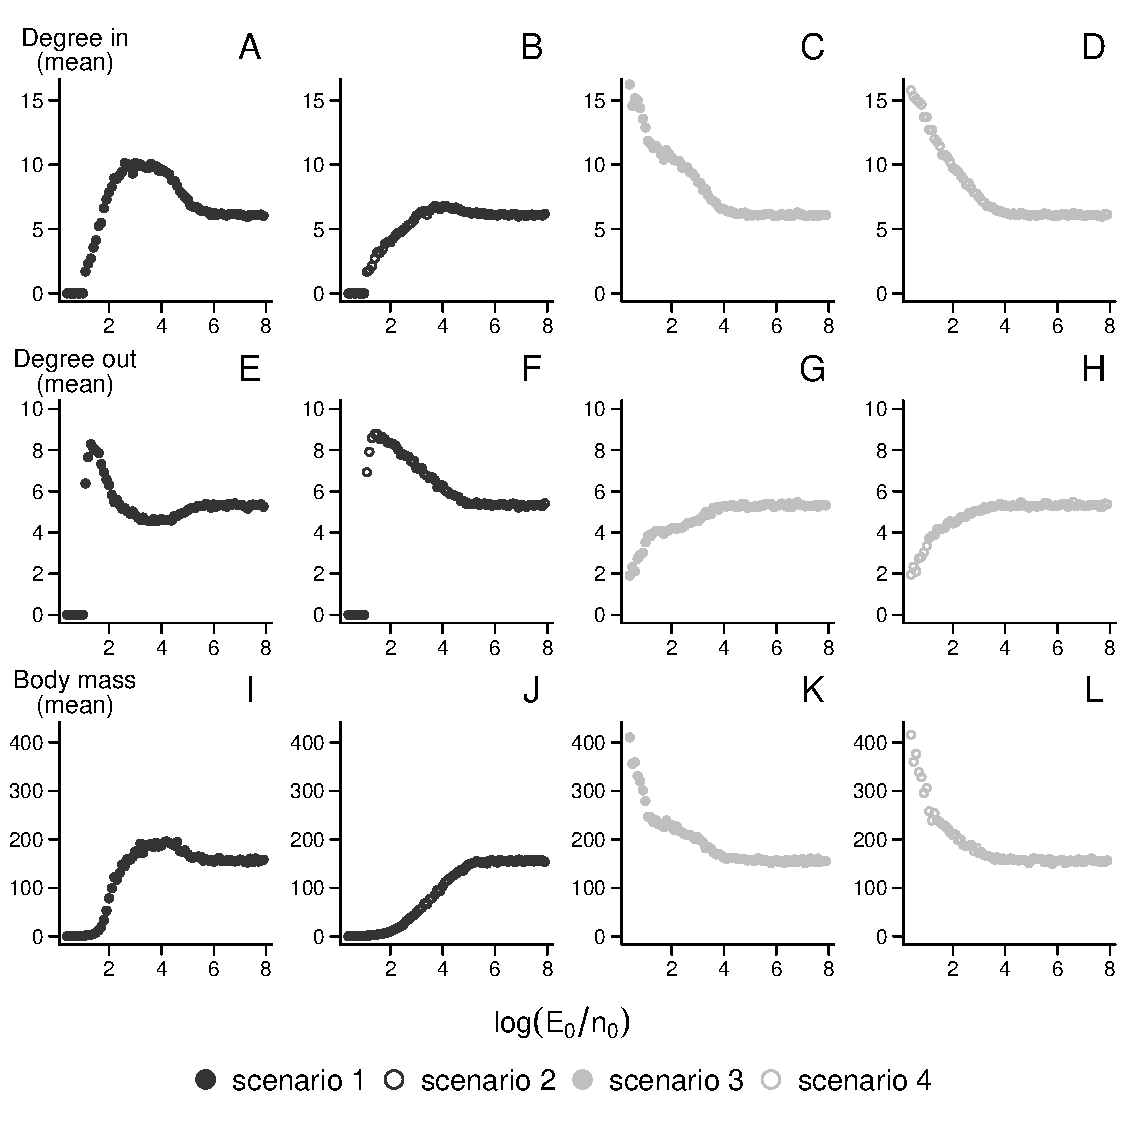
\includegraphics[width=\textwidth]{chapitre4/fig/fig4.pdf}
\caption[Average body mass, number of preys, predators of
predator species and the average number of interactions per species on
the island]{\textbf{Average body mass, number of preys, predators of
predator species and the average number of interactions per species on
the island} in regards to the energy gradient for four scenarios: (A)
A,E,I, (B) B, F, J, M (C) C, G, K, O and (D) D, H, L,
P.\label{fig:etib4}}
\end{figure}

The formulation of the TIB in terms of energy offers a great opportunity
to integrate to a mechanistic biogeography, one which strongly eases the
integration of various ecological processes. For example, here we show
how three ecological necessities are continually overlooked in classical
biogeographical theories: (1)- the necessity for a minimum population in
order to sustain presence on an island, (2)- the necessity of finding
resource/prey to maintain this population, and (3)- the difference in
energy uptake due to body mass and trophic level variations among
species. Based on this integration, we showed how the structure of the
community is constrained by the energy availability to the species in
question on islands. We also point out that the structure of the food
webs, which determines the energy requirements of the whole community,
controls the species richness and the characteristics of species
presence of the island.

In our study, we study the SER under two dfferent scenarios considering
the MVP either decreased with the body mass (C and D) or did not (A and
B). The results were qualitatively similar, however, were also
quantitatively different. In our first case, we find that larger species
can colonize earlier -- leading to increases in species richness for the
island. Where having a lower MVP for larger species can allow for energy
compensation costs associated with the maintenance of a larger body.
Furthermore, this could explain the ``energetic equivalence rules''
\citep{Nee1991} - species have an equal share of energy allocated
irrespective to their body mass \citep{Brown2003, Damuth2007}. In our
case, this holds true as long as the island is ``saturated'' with
species. Remarkably, under this condition, the relationship between the
logarithm of species richness and the logarithm of available energy
(\ref{fig:etib1} B) is linear, which is consistent with empirical
observations \citep[see Fig 3. and Fig 4. in][]{Wright1983}. Over
evolutionary scales, these observation would also be consistent with the
Ecological Limits hypothesis to diversification dynamics \citep{Rabosky2015}.

Our findings suggest that there is a clear relationship between the
trophic status of species and its occurrence probability: species of
higher trophic levels, irrespective of their body mass, colonize islands
with higher energy. This indicates that the food-chain length is limited
by the energy availability. Remarkably, a comparable relationship has
already been observed by \citet{Post2000}, who has found a correlation
among maximal food-chain length and lake size, which is consistent with
the idea that higher trophic level predators need larger areas that are
accompanied with sufficient amount of prey species in order to survive
in these lakes (larger area = more potential energy to consume).

Using our framework, we showed that under scenarios C and D (for which
MVP decreases with the body mass), generalist species are the first to
colonize the island. Remarkably, the early colonization of generalist
species has been highlighted by \citet{Piechnik2008} when they revisited
the classical study by \citet{Simberloff1969}. Also, reading Fig
\ref{fig:etib4} G-H in the direction of a loss of energy, we observe an
increase in generalist species similarly found by \citet{Clavel2011}.
The classical TIB has provided a theoretical basis for the SAR
\citep{MacArthur1967}, that has been largely used in conservation
practices to help determine the size of protected areas
\citep{Neigel2003}. However, as in the TIB, the SAR ignores the identity
of species, there is currently no theory integrating the position of a
species within the network it is embedded to predict its distribution.
The role of a species in the network must be of first importance to help
better understand the consequences of its loss \citep{Saterberg2013}.
The model we described here offers a testable hypothesis regarding the
role of the species that are expected to go extinct first, beginning
with the highest trophic level cascading to the lowest.

Finally, our framework is an opportunity to review the way we build
SDMs. Here, our model describes the food web dynamic associated to a
patch of primary producers. Fortunately, that primary production have
been proven highly correlated to climate variables
\citep{Wright1983, Hawkins2003, Evans2005} and are readily quantifiable
using indices such as the normalized difference vegetation index
\citep[NDVI,][]{Evans2005}. Here, such a quantity is not only a proxy to
assess the diversity of primary producers and their productivity, but
also a potential metric of the species richness \citep{Wright1983}, and
a predictor for network structure (\emph{e.g.} a predictor of the food
chain length for instance). Current species distribution models are
based on the correlations between abiotic factors and their occurrence
probabilities. It is described as a species abiotic niche, while its
presence could be best explained by the presence of its preys (see
chapter \ref{chap4}). Therefore, focusing on the prediction of the
distribution of primary producers while using information gathered
concerning the associated energy that they could provide to higher
trophic levels provides a promising avenue to enhance our understandings
of tomorrow's biodiversity.
